\documentclass{ifacconf}
%%%put this lines in ifacconf before hyperref to use it
\makeatletter
\let\old@ssect\@ssect % Store how ifacconf defines \@ssect
\makeatother
\usepackage{amsfonts,amssymb,amsmath,amsthm}

%% set-style letters
\def\AA{{\mathbb{A}}}
\def\BB{{\mathbb{B}}}
\def\CC{{\mathbb{C}}}
\def\DD{{\mathbb{D}}}
\def\EE{{\mathbb{E}}}
\def\FF{{\mathbb{F}}}
\def\GG{{\mathbb{G}}}
\def\HH{{\mathbb{H}}}
\def\II{{\mathbb{I}}}
\def\JJ{{\mathbb{J}}}
\def\KK{{\mathbb{K}}}
\def\LL{{\mathbb{L}}}
\def\MM{{\mathbb{M}}}
\def\NN{{\mathbb{N}}}
\def\OO{{\mathbb{O}}}
\def\PP{{\mathbb{P}}}
\def\QQ{{\mathbb{Q}}}
\def\RR{{\mathbb{R}}}
\def\SS{{\mathbb{S}}}
\def\TT{{\mathbb{T}}}
\def\UU{{\mathbb{U}}}
\def\VV{{\mathbb{V}}}
\def\WW{{\mathbb{W}}}
\def\XX{{\mathbb{X}}}
\def\YY{{\mathbb{Y}}}
\def\ZZ{{\mathbb{Z}}}

%% calligraphic letters
\def\cA{{\mathcal{A}}}
\def\cB{{\mathcal{B}}}
\def\cC{{\mathcal{C}}}
\def\cD{{\mathcal{D}}}
\def\cE{{\mathcal{E}}}
\def\cF{{\mathcal{F}}}
\def\cG{{\mathcal{G}}}
\def\cH{{\mathcal{H}}}
\def\cI{{\mathcal{I}}}
\def\cJ{{\mathcal{J}}}
\def\cK{{\mathcal{K}}}
\def\cL{{\mathcal{L}}}
\def\cM{{\mathcal{M}}}
\def\cN{{\mathcal{N}}}
\def\cO{{\mathcal{O}}}
\def\cP{{\mathcal{P}}}
\def\cQ{{\mathcal{Q}}}
\def\cR{{\mathcal{R}}}
\def\cS{{\mathcal{S}}}
\def\cT{{\mathcal{T}}}
\def\cU{{\mathcal{U}}}
\def\cV{{\mathcal{V}}}
\def\cW{{\mathcal{W}}}
\def\cX{{\mathcal{X}}}
\def\cY{{\mathcal{Y}}}
\def\cZ{{\mathcal{Z}}}
\def\cKL{{\mathcal{KL}}}

%% bold letters
\def\bA{{\bf{A}}}
\def\bB{{\bf{B}}}
\def\bC{{\bf{C}}}
\def\bD{{\bf{D}}}
\def\bE{{\bf{E}}}
\def\bF{{\bf{F}}}
\def\bG{{\bf{G}}}
\def\bH{{\bf{H}}}
\def\bI{{\bf{I}}}
\def\bJ{{\bf{J}}}
\def\bK{{\bf{K}}}
\def\bL{{\bf{L}}}
\def\bM{{\bf{M}}}
\def\bN{{\bf{N}}}
\def\bO{{\bf{O}}}
\def\bP{{\bf{P}}}
\def\bQ{{\bf{Q}}}
\def\bR{{\bf{R}}}
\def\bS{{\bf{S}}}
\def\bT{{\bf{T}}}
\def\bU{{\bf{U}}}
\def\bV{{\bf{V}}}
\def\bW{{\bf{W}}}
\def\bX{{\bf{X}}}
\def\bY{{\bf{Y}}}
\def\bZ{{\bf{Z}}}
\def\ba{{\bf{a}}}
\def\bb{{\bf{b}}}
\def\bc{{\bf{c}}}
\def\bd{{\bf{d}}}
\def\be{{\bf{e}}}
\def\boldf{{\bf{f}}} %different
\def\bg{{\bf{g}}}
\def\bh{{\bf{h}}}
\def\bi{{\bf{i}}}
\def\bj{{\bf{j}}}
\def\bk{{\bf{k}}}
\def\bl{{\bf{l}}}
\def\bm{{\bf{m}}}
\def\bn{{\bf{n}}}
\def\bo{{\bf{o}}}
\def\bp{{\bf{p}}}
\def\bq{{\bf{q}}}
\def\br{{\bf{r}}}
\def\bs{{\bf{s}}}
\def\bt{{\bf{t}}}
\def\bu{{\bf{u}}}
\def\bv{{\bf{v}}}
\def\bw{{\bf{w}}}
\def\bx{{\bf{x}}}
\def\by{{\bf{y}}}
\def\bz{{\bf{z}}}

%% other symbols
\DeclareMathOperator{\1}{\mathbf{1}}
\DeclareMathOperator{\0}{\mathbf{0}}
\DeclareMathOperator{\Id}{I}
\newcommand{\td}{\mathfrak{t}} % discrete-time 
\newcommand{\tr}{^\top}

%% operators
\DeclareMathOperator{\col}{col}
\DeclareMathOperator{\diag}{diag}
\DeclareMathOperator{\blkdiag}{blkdiag}
\DeclareMathOperator{\rank}{rank}
\DeclareMathOperator{\dis}{d}
\DeclareMathOperator{\sat}{sat} 
\DeclareMathOperator{\convhull}{\textbf{co}}
\DeclareMathOperator{\argmin}{argmin}
\DeclareMathOperator{\argmax}{argmax}
\DeclareMathOperator{\spec}{spec}
\def\He#1{\texttt{\rm{He}}\left\{{#1}\right\}}
\DeclareMathOperator{\trace}{tr}
\newcommand{\Imag}{\mathrm{Im}}

%% shortcuts
\newcommand{\norm}[1]{\lvert #1\rvert}
\newcommand{\wnorm}[2]{\lvert #1\rvert^2_{#2}}
\newcommand{\pderiv}[2]{\dfrac{\partial #1}{\partial #2}}
\newcommand{\pdef}[1]{\SS_{\succ0}^{#1}}
\newcommand\psemidef[1]{\SS_{\succeq0}^{#1}}
\newcommand{\bmx}[1]{\left[\begin{matrix}#1\end{matrix}\right]}
\newcommand{\pmx}[1]{\left(\begin{matrix}#1\end{matrix}\right)}
\newcommand{\smallpmat}[1]{\left(\begin{smallmatrix} #1 \end{smallmatrix} \right)}
\newcommand{\smallqmat}[1]{\left[\begin{smallmatrix} #1 \end{smallmatrix} \right]}
\newcommand{\overbar}[1]{\mkern 1.5mu\overline{\mkern-1.5mu#1\mkern-1.5mu}\mkern 1.5mu}
\renewcommand{\underbar}[1]{\mkern 1mu\underline{\mkern-1mu#1\mkern-1mu}\mkern 1mu}

\usepackage{hyperref}
\usepackage{graphicx}
\usepackage{float}

% SCRIPTS FOR DOUBLE AND SINGLE IMAGE

% \begin{figure}[H]
%     \centering
%     \begin{subfigure}{0.4\textwidth}
%     \includegraphics[width=\textwidth]{}
%     \caption{}
%     \label{}
%     \end{subfigure}
%     \hfill
%     \begin{subfigure}{0.55\textwidth}
%     \includegraphics[width=\textwidth]{}
%     \caption{}
%     \label{}
%     \end{subfigure}
%     \caption{}
%     \label{}
% \end{figure}

% \begin{figure}[H]
%     \centering
%     \includegraphics[width=0.65\textwidth]{}
%     \caption{}
%     \label{}
% \end{figure}

\usepackage{natbib}
%\usepackage{booktabs}
%%%put this lines in ifacconf after hyperref to use it
\makeatletter
\def\@ssect#1#2#3#4#5#6{%
  \NR@gettitle{#6}% Insert key \nameref title grab
  \old@ssect{#1}{#2}{#3}{#4}{#5}{#6}% Restore ifacconf's \@ssect
}
\makeatother

%%theorems
\theoremstyle{plain}
\newtheorem{theorem}{Theorem}
\newtheorem{proposition}{Proposition}
\newtheorem{assumption}{Assumption}
\newtheorem{lemma}{Lemma}
\newtheorem{remark}{Remark}
\newtheorem{definition}{Definition}
\newtheorem{corollary}{Corollary}
\newtheorem{problem}{Problem}
\newenvironment{proof}{\paragraph*{Proof:}}{\hfill$\square$}

\begin{document}
\begin{frontmatter}

\title{{\color{red}\textbf{TODO}}}

\author[First]{Marco Sterlini}
\author[Second]{Samuele Zoboli}
\author[Second]{Sophie Tarbouriech}

\address[First]{\color{red}\textbf{TODO}}
\address[Second]{\color{red}\textbf{TODO}}


\begin{abstract}
{\color{red}\textbf{TODO}}
\end{abstract}

\begin{keyword}
{\color{red}\textbf{TODO}}
\end{keyword}

\end{frontmatter}

\section{Introduction}
{\color{red}\textbf{TODO}}\\
\emph{Notation:} $\NN, \RR^{n}, \RR^{n \times m}$ denote the set of natural non-negative integers, the set of real vectors of dimension $n$ and the set of real matrices of dimension $n \times m$, respectively. For any matrix $A$, $A\tr$ is its transpose. For any square matrix $A$, the operator $\He{ A } = A + A\tr$ is defined. $\texttt{diag}(A_1, A_2)$ is a block-diagonal matrix with block-diagonal matrices $A_1$ and $A_2$. For a partitioned matrix, the symbol $\star$ stands for symmetric blocks. $\1_n = \bmx{1 & \dots & 1}\tr \in \NN^{n \times 1}$. We identify with subscript $i$ the $i$-th element of a vector or the $i$-th row of a matrix.

\section{Problem Formulation}
We consider the nonlinear discrete-time system stabilized by a Neural Network (NN) controller, as represented in Figure \ref{fig:first_scheme} and described by:
\begin{equation}
  x^{+} = A x + B \texttt{sat}(\bar{u}) + C \Phi(E x) + D d 
\end{equation}
where the saturation function \texttt{sat} is defined as:
$$
    \texttt{sat}(\bar{u}) = \texttt{sign}(\bar{u})\text{min}(|\bar{u}|, \widehat{u})
$$
here $\widehat{u}$ represents the limit of the input signal, $x \in \mathbb{R}^{n_x}$ is the state vector, $\bar{u} \in \mathbb{R}^{n_u}$ denotes the raw output of the controller, $d \in \mathbb{R}^{n_d}$ is a constant disturbance input, and $\Phi \in \mathbb{R}^{n_q}$ characterizes the nonlinearities of the system.
\begin{assumption}\label{ass:nonlin}
We assume that $\Phi$ satisfies some local quadratic abstraction for some $\underline{\mu}, \bar{\mu} > 0 \in \RR^{n_q}, \bar{S}, \bar{Q}, \bar{W} \in \RR^{n_q \times n_q}$
\begin{equation}\label{eqn:nonlin-set}
\forall v \in \bar{S} := \left\{ v \in  \RR^{n_q} : - \underline{\mu}_i \leq v_i \leq \bar{\mu}_i, i \in \pmx{1 & \dots & n_q} \right\} 
\end{equation}
\begin{equation}\label{eqn:nonlin-inclusion}
\bmx{x \\ \Phi(x)}\tr \bmx{\bar{S} & \bar{Q} \\ \star & \bar{W}} \bmx{x \\ \Phi(x)} \geq 0
\end{equation}
\end{assumption}\textcolor{red}{Please help in adding details about $\Phi$ since it's NOLCOS}.

\begin{figure}[H]
    \centering
    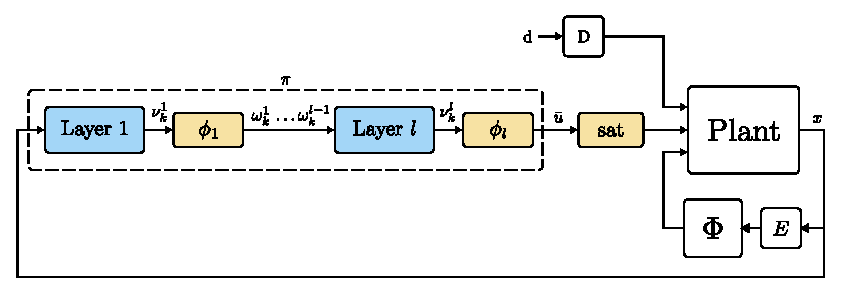
\includegraphics[width=0.45\textwidth]{Figures/first_scheme}
    \caption{Feedback system}
    \label{fig:first_scheme}
\end{figure}
The controller is implemented as a Multi-Layer Perceptron (MLP) with $l$ layers, each containing $n_{\phi_i}$ neurons for $i \in {1, \dots, l}$. All activation functions are saturation functions, represented by $\phi_i$. The goal is to design an Event-Triggering Mechanism (ETM) that alleviates the computational burden associated with evaluating numerous nonlinear activation functions while simultaneously providing sufficient sector conditions to manage the nonlinearities of both the system and the controller. The controller $\pi$ is defined as:
\begin{equation}\label{eqn:nn-equations}
  \begin{aligned}
  \widehat{\omega}^{0}(k) &= x(k) \\
  \nu^{i}(k) &= W^{i} \widehat{\omega}^{i - 1}(k) + b^{i}, i \in \left\{ 1, \dots, l \right\}\\
  \omega^{i}(k) &= \phi_i(\nu^i(k))\\
  \bar{u}(k) &= \phi_l(\nu^l(k))
  \end{aligned} 
\end{equation}
$\nu^i(k) \in \mathbb{R}^{n_{\phi_i}}$ represents the input to the $i$-th activation function $\phi^i: \mathbb{R}^{n_{\phi_i}} \to \mathbb{R}^{n_{\phi_i}}$, and $\omega^i(k), \widehat{\omega}^i(k) \in \mathbb{R}^{n_{\phi_i}}$ denote the current and last forwarded outputs, respectively. The weights $W^i \in \mathbb{R}^{n_{\phi_i} \times n_{\phi_{i-1}}}$ and biases $b^i \in \mathbb{R}^{n_{\phi_i}}$ define the affine transformation of each layer. The application of the saturation function is element-wise and is denoted as $\phi^i(\nu^i(k)) = \left[ \varphi(\nu^i_1(k)), \dots, \varphi(\nu^i_{n_{\phi_i}}(k)) \right]$, where $\varphi: \mathbb{R} \to \mathbb{R}$ is a scalar activation function that is assumed to be symmetric and identical for every neuron.

Following the notation in \cite{css-paper}, the controller policy is expressed in a condensed form. Introducing the augmented vectors:
\begin{equation*}
  \nu = \bmx{\nu^1 \\ \vdots \\ \nu^l}, \omega = \bmx{\omega^1 \\ \vdots \\ \omega^l}, \phi = \bmx{\phi^1(\nu^1) \\ \vdots \\ \phi^l(\nu^l)} 
\end{equation*}
With $n_{\phi} = \sum_{i=1}^{l} n_{\phi_i}$ and $\phi: \mathbb{R}^{n_{\phi}} \to \mathbb{R}^{n_{\phi}}$ representing the combined nonlinearity, we have $\omega = \phi(\nu)$. Finally, the conditions in \eqref{eqn:nn-equations} can be reformulated as:
\begin{equation*}
  \bmx{u(k)\\ \nu(k)} = \overbar N \bmx{x(k) \\ \omega(k) \\ 1} 
\end{equation*}
where
\begin{equation}\label{eqn:first-N}
  \overbar N := \bmx{
    \begin{array}{c | c c c c | c}
      \0 & \0 & \dots & \0 & W^l & b^l \\ 
      \hline
      W^1 & \0 & \dots & \0 & \0 & b^1 \\
      \0 & W^2 & \dots & \0 & \0 & b^2 \\
      \vdots & \vdots & \ddots & \vdots & \vdots & \vdots \\
      \0 & \0 & \dots & W^{l-1} & \0 & b^{l-1}
    \end{array}
  }
\end{equation}
Similarly to \cite{css-extended}, we implement an ETM in every layer of the controller, with an additional one at the output. This final ETM is designed to further reduce the total number of events and calls to the nonlinear functions. The system and controller are now represented in Figure \ref{fig:second_scheme}.
\begin{figure}[H]
    \centering
    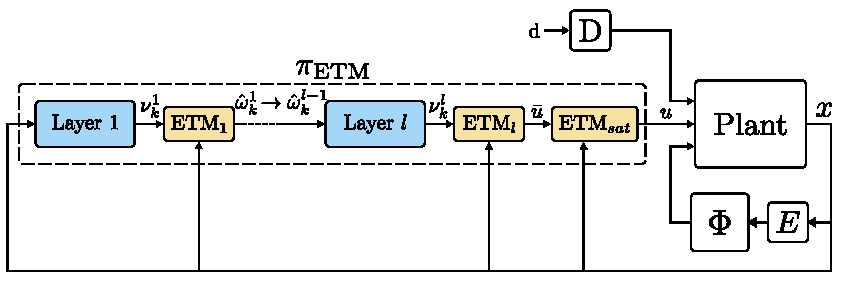
\includegraphics[width=0.45\textwidth]{Figures/second_scheme}
    \centering
    \caption{Feedback system subject to ETM in the controller}
    \label{fig:second_scheme}
\end{figure}

The system dynamics are rewritten as:
\begin{equation}\label{eqn:system-dynamics}
x^{+} = A x + B u + C \Phi(E x) + D d
\end{equation}
where $u \in \mathbb{R}^{n_u}$ is the output of the controller subject to the ETM. This modification requires redefining the matrix $\overbar N$, originally defined in the controller policy \eqref{eqn:first-N}, as:
\begin{equation}\label{eqn:last-N}
  N := \bmx{
    \begin{array}{c | c c c c | c}
      \0 & \0 & \dots & \0 & \Id & 0 \\ 
      \hline
      W^1 & \0 & \dots & \0 & \0 & b^1 \\
      \0 & W^2 & \dots & \0 & \0 & b^2 \\
      \vdots & \vdots & \ddots & \vdots & \vdots & \vdots \\
      \0 & \0 & \dots & W^l & \0 & b^l
    \end{array}
  } = \bmx{
    \begin{array}{c | c | c}
    N_{u x} & N_{u \omega} & N_{u b} \\
    \hline
    N_{\nu x} & N_{\nu \omega} & N_{\nu b}
    \end{array} 
  }
\end{equation}
The system adheres to the assumptions outlined in \citep[Lemma 2]{css-extended}, which allow us to derive the following expressions for the equilibrium points $\left( x_*, u_*, \nu_*, \omega_* \right)$ of the system and controller, given $x_*$. The matrices are defined as:
\begin{equation}
    \begin{aligned}
         &R = (\Id - N_{\nu \omega})^{-1}\\
         &R_{\omega} = N_{u x} + N_{u \omega} R N_{\nu x}\\
         &R_b = N_{u \omega} R N_{\nu b} + N_{u b}
    \end{aligned}
\end{equation}
Given the lower triangular structure of $N_{\nu \omega}$, the expression for $R$ is always invertible and exists. The equilibrium of the state is found using a numerical solver that minimizes the following expression, as it is no longer explicit due to the nonlinearity $\Phi$. Given a constant disturbance $\bar{d}$:
\begin{equation}
  x_* = \min_{x} \left[(A + B R_{\omega} - \Id) x + C \Phi(E x) + D \bar{d} + B R_b \right]
\end{equation}
\begin{equation}\label{eqn:equilibrium}
  \bmx{u_* \\ \nu_*} = N \bmx{x_* \\ \omega_* \\ 1}; \ \  
  \begin{aligned}
    \omega_* &= \nu_*\\
    \nu_* &= R N_{\nu x} x_* + R N_{\nu b}\\
    u_* &= R_{\omega} x_* + R_b
  \end{aligned}
\end{equation}
All the nonlinearities of the system and the controller are chosen to be saturation functions. In accordance with \citep[Lemma 3]{css-extended}, we state the local sector conditions that hold for every state within the following set:
\begin{remark}\label{rem:sec-set}
\emph{For $i \in \left\{ 1, \dots, l \right\}$ given a matrix $G^i \in \RR^{n_{\phi_i} \times n_x}$, if $x$ belongs to the set}
\begin{equation}\label{eqn:inclusion-set}
S := \left\{ x \in \RR^{n_x} : -\bar{\nu}^i - \bar{\nu}^i_* \leq G^i (x - x_*) \leq \bar{\nu}^i - \nu_*^i \right\} 
\end{equation}

\emph{Then the following quadratic constraint holds for any diagonal positive definite matrix $T^i \in \RR^{n_{\phi_i} \times n_{\phi_i}}$:}
\begin{equation}\label{eqn:first_sec_cond}
  \left[ \nu^i - \omega^i \right]\tr T^i \left[ G^i (x - x_*) - (\omega^i - \omega^i_*) \right] \leq 0
\end{equation}\end{remark}
Where $\bar{\nu}^i$ represents the saturation level of the $i$-th layer.

For ease of reference, the dead-zone vector is defined as $\psi^i = \nu^i - \omega^i$ and $\widehat{\psi}^i = \nu^i - \widehat{\omega}^i$. Additionally, all subsequent discussions will use incremental variables relative to their equilibrium, denoted with a tilde, i.e., $\tilde{x} = x - x_*$. Considering \eqref{eqn:equilibrium}, we have $\psi_* = \nu_* - \omega_* = 0$, hence $\tilde{\psi} = \psi$. We define $\xi^i = \begin{bmatrix} \tilde{x}^\top & \tilde{\psi}_i^\top & \tilde{\nu}_i^\top \end{bmatrix}^\top$ and $\widehat{\xi}^i = \begin{bmatrix} \tilde{x}^\top & \widehat{\tilde{\psi}}_i^\top & \tilde{\nu}_i^\top \end{bmatrix}^\top$. Then, the overall sector conditions \eqref{eqn:first_sec_cond} can be rewritten, with no loss of generality, for all $i \in {1, \dots, l}$ as:
\begin{equation}\label{eqn:sec_cond}
\begin{aligned}
    &({\tilde{\psi}^i})\tr T^i \bmx{G^i \tilde{x} + \tilde{\psi}^i - \tilde{\nu}^i} = {\xi^i}\tr \bmx{0 & 0 & 0\\
    T^i G^i & T^1 & -T^1\\
    0 & 0 & 0} \xi^i = \\
    &= {\xi^i}\tr \Omega^i \xi^i \leq 0
\end{aligned}
\end{equation}

\begin{remark}\label{rem:sec-cond}
Note that ensuring ${\xi^i}^\top \Omega^i \xi^i < 0$ guarantees that the sector condition \eqref{eqn:sec_cond} holds.
\end{remark}

We can now express the new interdependency between the variables of interest as follows:
\begin{equation}\label{eqn:incremental}
  \begin{aligned}
    \tilde{u} &= R_{\omega} \tilde{x} - N_{u \omega} R \tilde{\psi}\\
    \tilde{\nu} &= R N_{\nu x} \tilde{x} + (\Id - R) \tilde{\psi}
  \end{aligned}
\end{equation}

\section{Main Results}

Inspired by \citep[Proposition 1, Lemma 3]{css-extended}, we design the ETM for the output of each layer of the controller and the final output. This is achieved by first incorporating a dynamic threshold and then refining the triggering function using Finsler's lemma.

\subsection{Event-triggering mechanism}
An ETM operates by triggering an event to update the current layer and propagate its value throughout the network. In the previous work \cite{css-extended}, the triggering function was designed based on the saturation sector conditions in the form of \eqref{eqn:sec_cond}. The ETM was defined as:
\begin{equation}
  \widehat{\omega}^{i}(k) = \begin{cases}
    \phi^i(\nu^i(k)) & \text{if } {\widehat{\xi^i}}\tr \Omega^i \widehat{\xi^i} > 0\\
    \widehat{\omega}^{i}(k-1) & \text{otherwise}
  \end{cases}
\end{equation}
This approach functions as a static ETM, triggering an event immediately when the sector conditions are violated. Building upon the concepts from \cite{data-driven}, we propose a dynamic quantity to be incorporated into the ETM triggering condition. The goal is to reduce the conservatism of the controller by introducing a time-varying threshold that adapts to the current state of the system and controller, thereby decreasing the overall number of events and computational burden. The new triggering function for the proposed \emph{dynamic-ETM} for the $i$-th layer is defined as:
\begin{equation}\label{eqn:dynamic_trig}
  \widehat{\omega}^{i}(k) = \begin{cases}
    \phi^i(\nu^i(k)) & \text{if } {\widehat{\xi^i}}\tr \Omega^i \widehat{\xi^i} > \rho^i \eta_i\\
    \widehat{\omega}^{i}(k-1) & \text{otherwise}
  \end{cases};
\end{equation}

Where $\eta^i$ is characterized by the following dynamics:
\begin{equation}\label{eqn:eta_dynamics}
  {\eta^i}^+ = \rho^i \eta^i - {\widehat{\xi^i}}\tr \Omega^i \widehat{\xi^i}\quad  \forall i \in \left( 1, \dots, l \right) 
\end{equation}

We introduce a condensed notation that incorporates all conditions across each layer.
\begin{equation}
\begin{aligned}
   \bR &= \text{diag} \pmx{\rho^1 & \dots & \rho^l }\\
   \mathbf{\Psi} &= \bmx{ {\widehat{\xi^1}}\tr \Omega^1 \widehat{\xi^1} & \dots & {\widehat{\xi^l}}\tr \Omega^l \widehat{\xi^l}}\tr\\
   \boldsymbol{\eta} &= \bmx{ \eta^1 & \dots & \eta^l}\tr   
\end{aligned}
\end{equation}

The ETM triggering condition and dynamic thresholds' dynamics can be rewritten in an element-wise fashion as:
\begin{equation}
\begin{aligned}
    \boldsymbol{\eta}^+ &= \bR \boldsymbol{\eta} - \mathbf{\Psi}\\
    \mathbf{\Psi} &> \bR \boldsymbol{\eta}
\end{aligned}
\end{equation}

\subsection{Finsler Lemma application}
Following the implementation of the dynamic threshold, a further refinement of the triggering condition has been considered. Recalling the triggering condition:
$$
\widehat{{\xi^i}}\tr \Omega^i \widehat{\xi^i} > \rho^i \eta^i
$$
Intuitively, the smaller the left-hand side of the inequality, the fewer events will be triggered. However, the structure of $\Omega^i$ is inflexible due to its strict relationship with the sector condition expression. The following lemma addresses this limitation by introducing triggering matrices designed to ensure a lower update rate for each layer, leveraging Finsler's lemma:

\begin{lemma}\label{lem:finsler} \emph{Considering the triggering policy \eqref{eqn:dynamic_trig}, $R^i$ such that ${\xi^i}\tr = \!R^i \bmx{\tilde{x} & \tilde{\psi} & \tilde{\nu}}\tr\! = R^i \xi\tr$, with reference to the structure in \eqref{eqn:sec_cond} and assuming \eqref{eqn:incremental} holds for some $\underline{\xi}, \bar{\xi} \in \RR^{n_x + 2n_{\phi}}$ such that $\forall \xi \in \left[ \underline{\xi}, \bar{\xi}\right]$, if $\exists X^i \in\! \RR^{(nx + 2n_{\phi_i}) \times (nx + 2n_{\phi_i})},$ $N^i_1 \in \RR^{n_x \times n_{\phi_i}}, N^i_2, N^i_3 \in \RR^{n_{\phi_i} \times n_{\phi_i}}$ a diagonal matrix $T^i \succ 0 \in \RR^{n_{\phi_i} \times n_{\phi_i}}, G^i \in \RR^{n_{\phi_i} \times n_x}$ such that:
\begin{equation}\label{eqn:finsler}
     {R^i}\tr\! He\left\{X^i - \Omega^i\right\}\! R^i + He\left\{ \smallpmat{N^i_1\\ N^i_2\\ N^i_3}\! \pmx{R N_{\nu x} & \Id - R & -\Id}\right\} \preceq 0
\end{equation}
Then we have ${\xi^i}\tr X^i \xi^i \leq {\xi^i}\tr \Omega^i \xi^i$}
\end{lemma}

\begin{proof} By pre- and post-multiplying for $\xi$ the previous expression we end up with
$$
    {\xi^i}\tr\! He \!\left\{\!X^i \!-\! \Omega^i\right\} \xi^i + He\!\left\{ \xi\tr\! \smallpmat{N^i_1\\ N^i_2\\ N^i_3}\! \smallpmat{R N_{\nu x} & \Id - R & -\Id} \xi\! \right\}\! \leq 0
$$
By expanding the term $\pmx{R N_{\nu x} & \Id - R & -\Id} \xi$ we end up with condition \eqref{eqn:incremental}, meaning that the expression is reduced to
$$
    {\xi^i}\tr \He{X^i - \Omega^i} \xi^i \leq 0
$$
By further expanding the expression and noting that it eventually reduces to a scalar, for which the transpose is equivalent to itself, we obtain:
\begin{equation*}
\begin{aligned}
    &{\xi^i}\tr (X^i + {X^i}\tr) \xi^i \leq {\xi^i}\tr (\Omega^i + {\Omega^i}\tr) \xi^i\\
    &2 {\xi^i}\tr X^i\xi^i \leq 2 {\xi^i}\tr \Omega^i \xi^i\\
    & {\xi^i}\tr X^i \xi^i \leq {\xi^i}\tr \Omega^i \xi^i
\end{aligned}
\end{equation*}
\end{proof}

Given $X^i$ matrices $i \in \left\{1, \dots, l \right\}$, we can rewrite the triggering conditions for each layer as:
\begin{equation}\label{eqn:etm-trigger}
  \widehat{\omega}^{i}(k) = \begin{cases}
    \phi^i(\nu^i(k)) & \text{if } {\xi^i}\tr X^i \xi > \rho^i \eta^i(k)\\
    \widehat{\omega}^{i}(k-1) & \text{otherwise}
  \end{cases}
\end{equation}
\begin{remark}\label{rem:eta-positive} \emph{Similarly to \citep[Lemma 3]{data-driven}, it can be demonstrated that $\eta^i$, the dynamic threshold of layer $i$, is always non-negative for any $\rho^i \in [0, 1)$, with the initial condition $\eta^i_0 \geq 0$.} \end{remark}
With respect to \eqref{eqn:etm-trigger} and \eqref{eqn:eta_dynamics} we have two possible occurrences:
\begin{itemize}
    \item $\widehat{{\xi^i}}\tr X^i \widehat{\xi^i} \leq \rho^i \eta^i$: It is trivial to verify that ${\eta^i}^+ = \rho^i \eta^i - \widehat{{\xi^i}}\tr X^i \widehat{\xi^i} \geq 0 $
    \item $\widehat{\xi^i}\tr X^i \widehat{\xi^i} > \rho^i \eta^i$: In this case, an event is triggered, and the vector $\widehat{\xi^i}$ gets updated to $\xi^i$ after the activation function application. In this situation, \eqref{eqn:sec_cond} is satisfied, and, with respect to Remark \ref{rem:sec-cond} and Lemma \ref{lem:finsler}, we have ${\xi^i}^\top X^i \xi^i < {\xi^i}^\top \Omega^i \xi^i < 0$. Once again, we have ${\eta^i}^+ = \rho^i \eta^i - {\xi^i}^\top X^i \xi^i > 0$.
\end{itemize}
By denoting 
\begin{equation}
    \bX = \text{diag} \pmx{{R^1}\tr X^1 R^1 & \dots & {R^l}\tr X^l & R^l}, \qquad \xi = \bmx{\tilde{x} \\ \tilde{\psi} \\ \tilde{\nu}}
\end{equation}
\begin{equation}\label{eqn:final-psi}
    \mathbf{\Psi_x} = \pmx{\Id_l \otimes \xi}\tr\! \bX \pmx{\1_l \otimes \xi}
\end{equation}
The ETM triggering condition and the dynamics of the dynamic thresholds can be rewritten in an element-wise fashion as:
\begin{equation}
\begin{aligned}
    \boldsymbol{\eta}^+ &= \bR \boldsymbol{\eta} - \mathbf{\Psi_x}\\
    \mathbf{\Psi_x} &> \bR \boldsymbol{\eta}\end{aligned}
\end{equation}

\subsection{Lyapunov conditions}
In this section, we will provide sufficient conditions for the stability of the system and controller in the form of Linear Matrix Inequalities (LMIs), ensuring local asymptotic stability. The solution to the problem will also yield the matrices $X^i$ and the parameters $\rho^i$ to be used in the ETM triggering conditions, along with an estimate of the Region of Attraction (ROA) for the equilibrium point.

We will first introduce a more compact notation for the system dynamics, along with some auxiliary matrices:
\begin{equation}\label{eqn:auxiliary}
\begin{aligned}
    &\bar{A} = A + B R_{\omega}\\
    &\bar{B} = -B N_{u \omega} R\\
    &\tilde{x}^+ = \bar{A}\tilde{x} + \bar{B}\tilde{\psi} + C \tilde{\Phi}\\
&R_{\nu} = \bmx{
  \Id & 0 & 0 \\
  0 & \Id & 0 \\
  R N_{\nu x} & \Id - R & 0\\
} \in \RR^{(n_x + n_{\phi} + n_q) \times (n_x + 2 n_{\phi})}\\
&R_s \in \RR^{(n_x + n_{\phi} + n_q) \times (n_x + n_q)}
\end{aligned}
\end{equation}

\begin{figure*}
\begin{subequations}\label{eqn:LMI}
\begin{align}\label{eqn:lyapunov}
  &\Xi =\bmx{
  \begin{array}{c|c}
  \bmx{\bar{A}\tr\\
  \bar{B}\tr\\
  C\tr
  } P \bmx{\bar{A} & \bar{B} & C} - \bmx{
  P & 0 & 0\\
  0 & 0 & 0\\
  0 & 0 & 0
  } - (\1_l \otimes R_{\nu})\tr \He{\bX} (\1_l \otimes R_{\nu})
   + R_s\tr \bmx{
    S & Q\\
    \star & W
  }  R_s\hspace{.1em}& 0\\[1.5em]
\hline \\[-0.9em]
  0 & \hspace{.1em} 2 (\bR - \Id)
  \end{array}} \prec 0\\
  &\bmx{
    P & {Z_j^i}\tr\\
    \star & 2 \alpha T^i_{j,j} - \alpha^2 (\widehat{\nu}_j^i)^{-2}
  } \succeq 0 \qquad \forall i \in \left\{ 1, \dots, l \right\}, j \in \left\{ 1, \dots, n_{\phi_i} \right\} \label{eqn:inclusion}\\
  &{R^i}\tr\! \He{X^i - \Omega^i} R^i + He\left\{ \pmx{N^i_1\\ N^i_2\\ N^i_3} \pmx{R N_{\nu x} & \Id - R & -\Id}\right\} \preceq 0 \qquad \forall i \in \left\{ 1, \dots, l \right\} \label{eqn:finsler_constraint}\\
  &\bmx{P & {E_i}\tr \\ \star & \widehat{\mu_i}^2} \succeq 0 \qquad \forall i \in \left\{1, \dots, n_q \right\} \label{eqn:nonlin-inclusion-constraint}
\end{align}
\end{subequations}
\vspace{.5em}
\hrule
\end{figure*}
% \begin{figure*}
% \begin{equation}\label{eqn:first-step}
%  \bmx{\tilde{x} \\ \tilde{\psi} \\ \tilde{\Phi}}\tr \left( \!
%   \bmx{\bar{A}\tr\\
%   \bar{B}\tr\\
%   C\tr
%   } P \bmx{\bar{A} & \bar{B} & C} - \bmx{
%   P & 0 & 0\\
%   0 & 0 & 0\\
%   0 & 0 & 0
%   } \right) \bmx{\tilde{x} \\ \tilde{\psi} \\ \tilde{\Phi}}
%  - \pmx{\1_l \otimes \xi}\tr \He{\bX} \pmx{\1_l \otimes \xi}
%  + \bmx{\tilde{x}\\ \tilde{\Phi}}\tr\! \bmx{S & Q\\ \star & W} \bmx{\tilde{x} \\ \tilde{\Phi}}
%  + \sqrt{\boldsymbol{\eta}}\tr \He{\bR - \Id} \sqrt{\boldsymbol{\eta}}
% \end{equation}
% \vspace{.5em}
% \hrule
% \end{figure*}

\begin{theorem}\label{thm:stability} \emph{ Consider the control system in \eqref{eqn:system-dynamics} and the controller $\pi_{\text{ETM}}$ in \eqref{eqn:nn-equations}. Assuming the existence of the matrices $P = P\tr \succ 0 \in \RR^{n_x \times n_x}$,} $T = \text{diag} \pmx{T^1 & \dots & T^l} \in \RR^{n_{\phi} \times n_{\phi}} \succ 0$, \emph{$Z = \smallpmat{{Z^1}\tr & \dots & {Z^l}\tr}\tr \in \RR^{n_{\phi} \times n_x}$, $\bR > 0$, $\bX$, $N^i_1, N^i_2, N^i_3 \ \forall i \in \left\{ 1, \dots, l \right\}$, $S \in \RR^{n_x \times n_x}, Q \in \RR^{n_x \times n_q}, W \in \RR^{n_q \times n_q}$ and a scalar $\alpha > 0$ such that the matrix inequalities \eqref{eqn:lyapunov}, \eqref{eqn:inclusion}, \eqref{eqn:finsler} hold, where $\widehat{\nu}_j^i = \min(|-\bar{\nu}_j^i - \nu^i_{*, j}|,|\bar{\nu}_j^i - \nu^i_{*, j}|)$, $
\widehat{\mu}_i = \min(|-\underline{\mu}_i - v_i^*|,|\bar{\mu}_i - v_i^*|)$ and $G^i = (T^i)^{-1} Z^i\ \forall i \in \left\{1, \dots, l \right\}$
Then the point $(x, \boldsymbol{\eta}) = (x_*, \0)$ is Locally Exponentially Stable (LES) with a ROA that includes the ellipsoid $\cE(P, x_*) = \left\{ x \in \RR^{n_x}, \boldsymbol{\eta} \in \RR^{l} : \tilde{x}\tr P \tilde{x} + \He{\1_l\tr \boldsymbol{\eta}} \leq 1\right\}$}
\end{theorem}


\begin{proof}
By exploiting the inequality $$\bmx{\alpha (\widehat{\nu}^i_j)^{-2} - T^i_{j, j}}(\widehat{\nu}^i_j)^2\bmx{\alpha (\widehat{\nu}^i_j)^{-2} - T^i_{j, j}} \geq 0$$ having $(T^i_{j,j})^2(\widehat{\nu}^i_j)^2 \geq 2 \alpha T^i_{j,j} - \alpha^2 (\widehat{\nu}_j^i)^{-2}$, and assuming \eqref{eqn:inclusion}, we state:
$$
\bmx{
P & (T^i_{j,j} G^i_j)\tr\\
\star & (T^i_{j,j})^2(\widehat{\nu}^i_j)^2
} \succeq 
\bmx{
P & {Z_j^i}\tr\\
\star & 2 \alpha T^i_{j,j} - \alpha^2 (\widehat{\nu}_j^i)^{-2}
} \succeq 0
$$
That implies
$$
\bmx{
P & 0 & (T^i_{j,j} G^i_j)\tr\\
0 & 2 \Id & 0\\
\star & 0 &(T^i_{j,j})^2(\widehat{\nu}^i_j)^2
} \succeq 0
$$
We initially assume the positivity of $\boldsymbol{\eta}$, by pre- and post-multiplying for $\bmx{\tilde{x}\tr, \sqrt{\boldsymbol{\eta}}, 1}\tr$ and its transpose, and applying Schur's complement, we obtain
$$
\bmx{\tilde{x}\\ \sqrt{\boldsymbol{\eta}}}\tr \bmx{P & 0\\ 0 & 2 \Id} \bmx{\tilde{x}\\ \sqrt{\boldsymbol{\eta}}} \succeq \tilde{x}\tr \frac{(G^i_j)\tr (G^i_j)}{\widehat{\nu^i_j}^2} \tilde{x}
$$
This ensures $\cE(P, x_*) \subseteq S$, as defined in Remark \ref{rem:sec-set}. Now, assuming \eqref{eqn:finsler_constraint} holds for all $(x, \boldsymbol{\eta}) \in \cE(P, x_*)$, the application of Lemma \ref{lem:finsler} guarantees that $\boldsymbol{\eta} > 0$ as discussed in Remark \ref{rem:eta-positive}. Considering \eqref{eqn:nonlin-inclusion-constraint}, we have:
$$
\bmx{P & 0 & E_i\tr \\
0 & 2 \Id & 0 \\
E_i & 0 & \widehat{\mu_i}^2} \succeq 0
$$
By expressing $v_i = E_i x$ and pre- and post-multiplying by $\bmx{\tilde{x}\tr & \tilde{\Phi}(Ex)\tr}\tr$ we have:
$$
\bmx{\tilde{x}\\ \sqrt{\boldsymbol{\eta}}}\tr \bmx{P & 0\\ 0 & 2 \Id} \bmx{\tilde{x}\\ \sqrt{\boldsymbol{\eta}}} \succeq \tilde{x}\tr \frac{E_i\tr E_i}{\widehat{\mu_i}^2} \tilde{x} = \frac{v_i\tr v_i}{\widehat{\mu_i}^2} \succeq 0
$$
Once again, this ensures $\cE(P, x_*) \subseteq \bar{S}$ as defined in Assumption \ref{ass:nonlin}, and thus $\cE(P, x_*) \subseteq \left\{ S \cap \bar{S} \right\}$.

We can define the following positive-definite candidate Lyapunov function structured as: $V = \tilde{x}\tr P \tilde{x} + \He{\1_l\tr\!\boldsymbol{\eta}}$. 
By denoting $R_s$ as a proper transformation matrix such that $\bmx{\tilde{v}\tr & \tilde{\Phi}(Ex)\tr}\tr = R_s \! \bmx{\tilde{x}\tr & \tilde{\psi}\tr & \tilde{\Phi}(Ex)\tr}\tr$ the following holds for all $x \in \cE(P, x_*)$:
\begin{equation}\label{eqn:sector-sign}
\bmx{\tilde{x} \\ \tilde{\psi} \\ \tilde{\Phi}(Ex)}\tr \! R_s\tr \! \bmx{S & Q \\ \star & W} R_s \bmx{\tilde{x} \\ \tilde{\psi} \\ \tilde{\Phi}(Ex)} \geq 0
\end{equation}
With respect to \eqref{eqn:auxiliary} and \eqref{eqn:incremental} by denoting \\$\xi = R_{\nu} \bmx{\tilde{x}\tr & \tilde{\psi}\tr & \tilde{\Phi}(Ex)\tr}\tr = R_{\nu} \zeta$, if we pre- and post-multiply \eqref{eqn:lyapunov} by $\bmx{\zeta\tr & \sqrt{\boldsymbol{\eta}}\tr}\tr$ and its transpose,we can express the intermediate term as follows: 
\begin{equation}
\begin{aligned}
  &\zeta\tr \pmx{\1_l \otimes R_{\nu}}\tr \He{\bX} \pmx{\1_l \otimes R_{\nu}} \zeta = \\
  =& \pmx{\1_l 1 \otimes R_{\nu} \zeta}\tr \He{\bX} \pmx{\1_l 1 \otimes R_{\nu} \zeta} = \\
  =& \pmx{\1_l \otimes \xi}\tr \He{\bX} \pmx{\1_l \otimes \xi} = \\
  =& \1_l\tr \pmx{\Id_l \otimes \xi}\tr \He{\bX} \pmx{\1_l \otimes \xi} = \1_l\tr \mathbf{\Psi_x}
\end{aligned}
\end{equation}
Considering \eqref{eqn:sector-sign}, we verify Assumption \ref{ass:nonlin}. Then, by collecting the appropriate terms for all $(x, \boldsymbol{\eta}) \in \cE(P, x_*)$ we have:
\begin{equation}
\begin{aligned}
&\bmx{\tilde{x} \\ \tilde{\psi} \\ \tilde{\Phi}}\tr \left( \!
  \bmx{\bar{A}\tr\\
  \bar{B}\tr\\
  C\tr
  } P \bmx{\bar{A} & \bar{B} & C} - \bmx{
  P & 0 & 0\\
  0 & 0 & 0\\
  0 & 0 & 0
  } \right) \bmx{\tilde{x} \\ \tilde{\psi} \\ \tilde{\Phi}} + \\
  &+ \He{\1_l\tr \bmx{(\bR - \Id) \boldsymbol{\eta} - \mathbf{\Psi_x}}} = \\
  &= (\tilde{x}^+)^{\top} P \tilde{x}^+ - \tilde{x}\tr P \tilde{x} + \He{\1_l\tr (\boldsymbol{\eta}^+ - \boldsymbol{\eta})} = \Delta V < 0, 
\end{aligned}
\end{equation}
Therefore, $\cE(P, x_*)$ is forward invariant, and all trajectories starting inside such a set converge to $(x, \0)$, thus concluding the proof.
\end{proof}
\begin{table*}[t]
    \centering
    \begin{tabular}{c|cccc|c|c|c}
    Setup & $\lambda_{l1}$  & $\lambda_{l2}$ & $\lambda_{l3}$ & $\lambda_u$ & $\lambda_{\text{tot }}$& $\VV (\cE(P, x_*))$ & $n_{\text{steps}}$\\
    \hline
    $\cS 1$ & $96.28$ & $54.80$ & $44.58$ & $28.17$ & $64.84$ & $80.28$ & $323$\\
    $\cS 2$ & $74.19$ & $40.65$ & $35.48$ & $30.32$ & $49.90$ & $65.78$ & $310$\\
    $\cS 3$ & $55.53$ & $36.70$ & $32.88$ & $21.29$ & $41.49$ & $81.34$ & $2278$\\
    $\cS 4$ & $44.90$ & $38.13$ & $35.61$ & $24.64$ & $39.39$ & $80.89$ & $2098$\\
    \end{tabular}
    \caption{Average results for $20$ simulations with different setups}
    \label{tab:results}
\vspace{.5em}
\hrule
\end{table*}
\subsection{Optimization procedure}
We now state a corollary whose results will be useful for deriving performance upgrades that will be discussed later.

\begin{corollary}\label{cor:optimization}
  \emph{Given Theorem \ref{thm:stability}, considering the decision variables $\Sigma, P, T, Z, \bX, \bR, S, Q, W, N^1_i, N^2_i, N^3_i, \beta_i \quad \forall i \in \left\{ 1, \dots, l \right\}$ with $\Sigma$ being a diagonal matrix $\Sigma > 0 \in \RR^{(n_x + 2 n_{\phi} + n_q) \times (n_x + 2 n_{\phi} + n_q)}$, and $\beta_i$ being scalars with the following optimization scheme:}
  \begin{equation}\label{eqn:optimization}
  \begin{aligned}
    &\min \trace{P} + \trace{\Sigma} + \sum_{i=1}^{l} \beta_i\\
    &\text{subject to } \eqref{eqn:LMI},\\ 
    &\qquad \qquad \Xi + \Sigma \succeq 0,\\
    &\qquad \qquad \bmx{-\beta_i \Id & X^i\\
    {X^i}\tr & -\Id} \preceq 0 \qquad i \in \left\{ 1, \dots, l \right\}
  \end{aligned}
  \end{equation}
  \emph{Then $(x_*, \0)$ is LES and $\cE(P, x_*)$ is an inner approximation of the ROA.}
\end{corollary}

By adding these constraints, we obtain the following performance upgrades:
\begin{itemize}
  \item Minimizing the trace of $P$ maximizes the volume of the ellipsoid $\cE(P, x_*)$, thereby increasing the Region of Attraction (ROA).
  \item Minimizing the trace of $\Sigma$ reduces the conservatism of the controller by obtaining a constraint matrix $\Xi$ that is directly related to the decay rate of the Lyapunov function, as close to zero as possible but never greater due to the second condition in \eqref{eqn:optimization}.
  \item Applying the Schur complement to the last condition in \eqref{eqn:optimization}, we obtain:
  $$
  || X^i || \preceq \beta_i \Id \qquad \forall i \in \left\{1, \dots, l \right\}
  $$
 This means that the smaller the value of $\beta_i$, the smaller the triggering function in the ETM \eqref{eqn:etm-trigger}, thus reducing the number of events.
\end{itemize}

It is important to comment on the quantity $\alpha$ in \eqref{eqn:inclusion}. If $\alpha$ were treated as a variable, the statements of Theorem \ref{thm:stability} would not hold as LMI conditions because bilinear terms would arise. To address this, we fix $\alpha$ to a constant value. The selection of $\alpha$ is important, as it directly influences the conservatism of the solution. To find a good value for $\alpha$, we use a \emph{golden ratio search algorithm}. This approach is based on the bisection method, with some basic improvements to enhance efficiency.

\begin{itemize}
  \item It reduces the number of LMI solutions required by efficiently narrowing the search interval.
  \item It maintains a constant reduction factor for the interval size, leading to more consistent progress towards the optimal value.
  \item It is particularly effective for unimodal functions, such as the one we encounter when optimizing the volume of the Region of Attraction (ROA).
\end{itemize}

\section{Simulations}
We considered an inverted pendulum system with mass $m = 0.15 kg$, length $l = 0.5 m$, damping coefficient $\mu = 0.05 N ms/rad$, gravitational acceleration $g = 9.81 m/s^2$. Additionally, an integrator is added to the system's dynamics. The discrete-time (DT) model of the system is given in the form of \eqref{eqn:system-dynamics} as:
\begin{equation}\label{eqn:pendulum}
\begin{aligned}
  &x = \bmx{\theta \\ \dot{\theta} \\ z} \quad 
  A = \bmx{1 & dt & 0\\
  \frac{g}{l} dt & 1 - \frac{\mu}{m l^2} dt & 0\\
  1 & 0 & 1}\quad
  B = \bmx{0\\ \frac{\bar{\tau}}{m l^2} dt\\ 0} \\
  &C = \bmx{0 \\ \frac{g}{l} dt \\ 0} \quad
  D = \bmx{0 \\ 0 \\ -1} \quad
  E = \bmx{1 & 0 & 0}
\end{aligned}
\end{equation}
With the maximum torque available $\bar{\tau} = 5 N m$, the sampling time $dt = 0.02 s$ and the nonlinearity $\Phi(Ex) = \text{sin}(Ex) - Ex$, proper quadratic abstractions to handle this nonlinearity have are already been explored in the literature, such as in \citep{junnarkar2024synthesizing}, which uses:
$$
\bmx{y\\sin(y) - y}\tr \bmx{0 & -1 \\ -1 & -2} \bmx{y\\sin(y)-y} > 0 \qquad \forall y \in \bmx{-\pi, \pi}
$$
Considering the system under examination, due to the periodicity of the $sin$ function, the previous conditions hold globally. By selecting $n_q = 1, S = 0, Q = -1, W=-2$, we avoid adding condition \eqref{eqn:nonlin-inclusion-constraint} in the LMI problem formulation.
A stabilizing NN controller was trained using Reinforcement Learning (RL), structured as an MLP of $3$ layers each having $n_{\phi_1} = n_{\phi_2} = n_{\phi_3} = 32$ neurons. The addition of the integrator in the system dynamics makes the training less trivial, enabling compensation for the intrinsic equilibrium points of the controller, which are typically different from the origin. The constroller's output $\bar{u}$ is a scalar, and the saturation level $\widehat{u}$ of the last ETM (see fig. \ref{fig:second_scheme}) is set to $1$, due to the nature of RL training, which always normalizes the final output of the network. By imposing $\alpha = 0.053$ we solved the LMI for 4 significant setups:
\begin{itemize}
    \item $\cS 1$: Old triggering conditions with static ETM minimizing $\trace{P}$ 
    \item $\cS 2$: Old triggering conditions with dynamic ETM minimizing $\trace{P} + \trace{\Sigma}$
    \item $\cS 3$: New triggering conditions minimizing $\trace{P} + \trace{\Sigma}$
    \item $\cS 4$: New triggering conditions minimizing $\trace{P} + \trace{\Sigma} + \sum_{i=1}^l \beta_i$
\end{itemize}
In Table \ref{tab:results}, the novelties and upgrades of the proposed method are highlighted. The data comes from the average of simulations starting from $20$ initial configurations such that $(x_0, \boldsymbol{\eta}_0) \in \cE(P_{\cS 2}, x_*)$, which corresponds to the more conservative result. The simulations are stopped whenever the Lyapunov function reaches an arbitrary small threshold, $10^{-15}$ in our case. The update rates are denoted by $\lambda_{li}$ and $\lambda_{\text{tot}}$, representing the percentage of the $i$-th layer and the overall controller respectively. Their expression follows:
$$
\lambda_{li} = \frac{n_{\text{events}_i}}{n_{\text{steps}}} \cdot 100; \qquad \lambda_{\text{tot}} = \frac{\sum_{i=1}^l \lambda_{li} \cdot n_{\phi_i}}{l}
$$
The volume of the ellipsoid $\cE(P_{\cC_i}, x_*)$ is a direct indication of the conservatism of the solution and is computed as:
$$
\VV(\cE(P_{\cC_i}, x_*) = \frac{4}{3} \frac{\pi}{\sqrt{\det P_{\cC_i}}}
$$
Finally, we analyze the number of simulation steps required to reach the previously mentioned threshold. A considerable decrease in the update rate of the controller is observed with every proposed method, accompanied by a more uniform event pattern across the different layers. The increased conservatism observed in $\cS 2$ is counterbalanced by the introduction of $X^i$ matrices in Lemma \ref{lem:finsler}, which leads to a larger ROA approximation and an improved update profile. $\cS 4$ represents a performance trade-off compared to $\cS 3$ in terms of computational savings and ellipsoid size. Both $\cS 3$ and $\cS 4$ maintain a low value for $\lambda_{\text{tot}}$ while having higher $n_{\text{steps}}$, indicating that the raw number of events is low, leading to more efficient event-triggering and fewer updates.

The following plots refer to $\cS 4$ with $$
x_0 = \bmx{-9.43(deg) \\ 5.77(rad/s) \\  0.0}; \quad \boldsymbol{\eta}_0 = 0.01 \cdot \1; \quad d = 2.76(deg)$$ 
as initial configuration.

\begin{figure}[H]
    \centering
    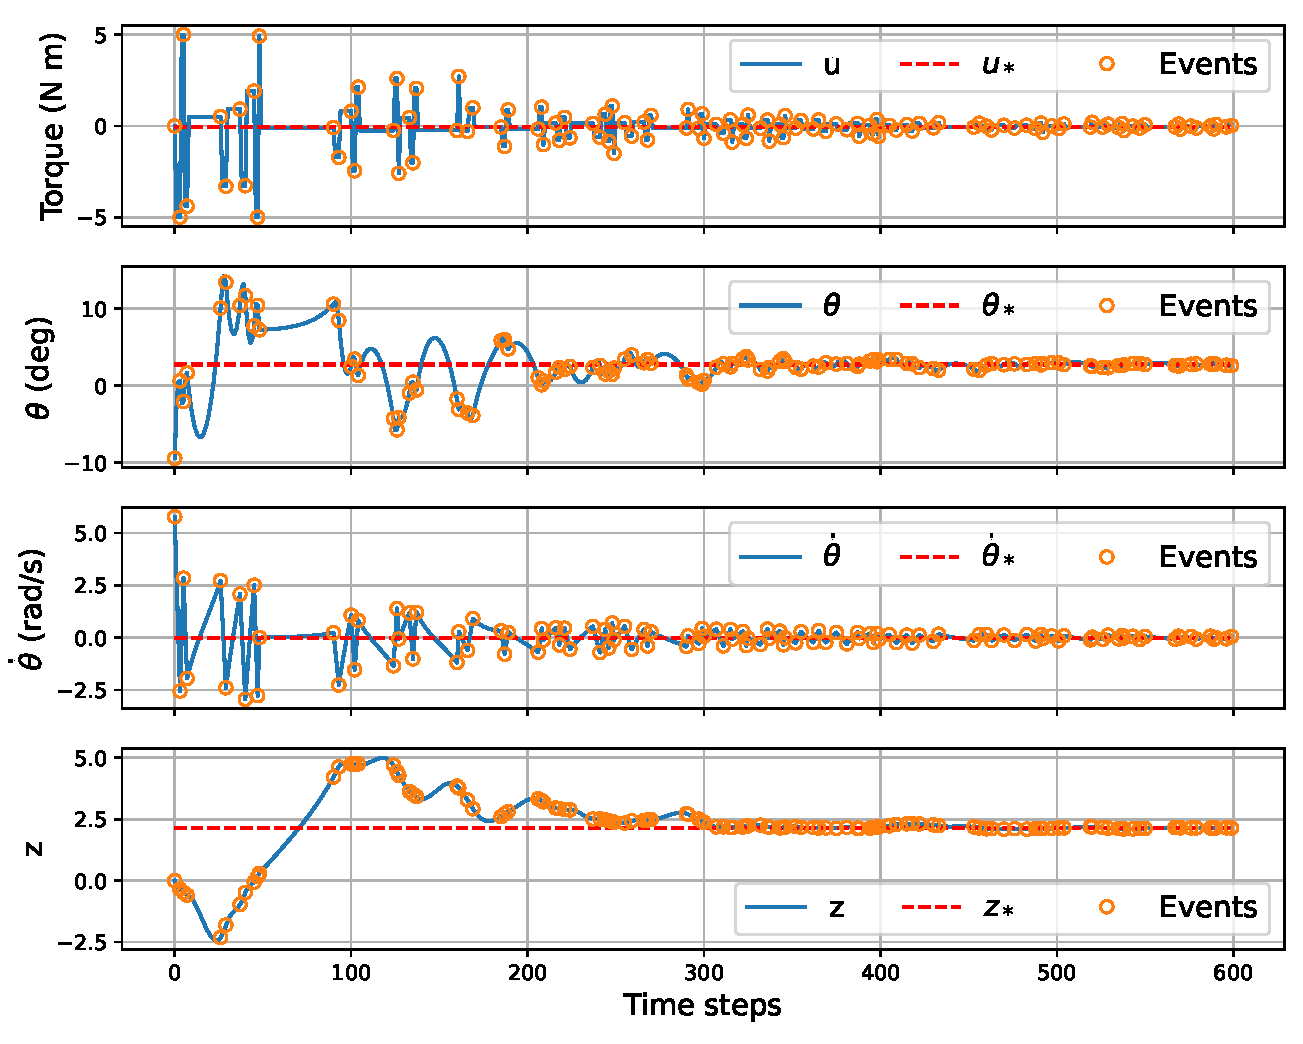
\includegraphics[width=0.45\textwidth]{Figures/evolution_plot}
    \caption{First $600$ steps evolution of $u, x$}
    \label{fig:evolution}
\end{figure}

\begin{figure}[H]
    \centering
    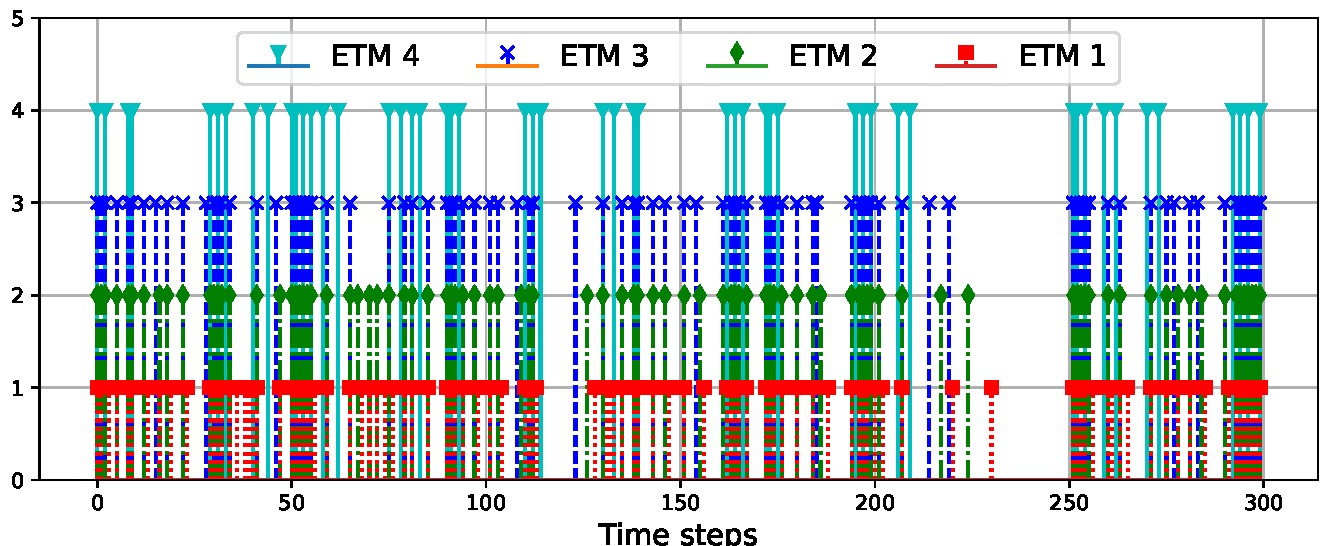
\includegraphics[width=0.45\textwidth]{Figures/event_plot}
    \caption{Events occurring in first $300$ steps}
    \label{fig:events}
\end{figure}

\begin{figure}[H]
    \centering
    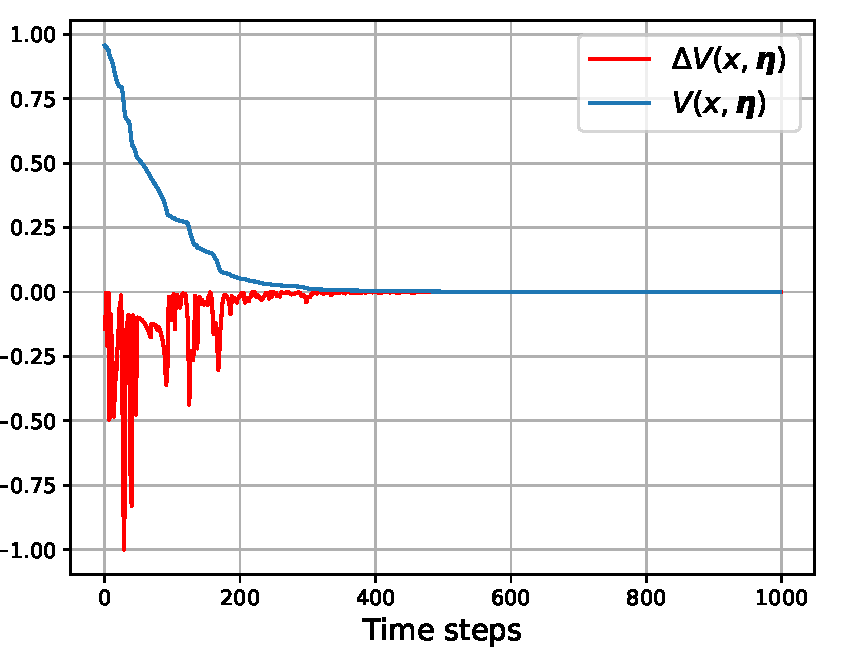
\includegraphics[width=0.45\textwidth]{Figures/lyapunov_plot}
    \caption{First $1000$ steps evolution of $V$ and normalized $\Delta V$}
    \label{fig:lyapunov}
\end{figure}

\begin{figure}[H]
    \centering
    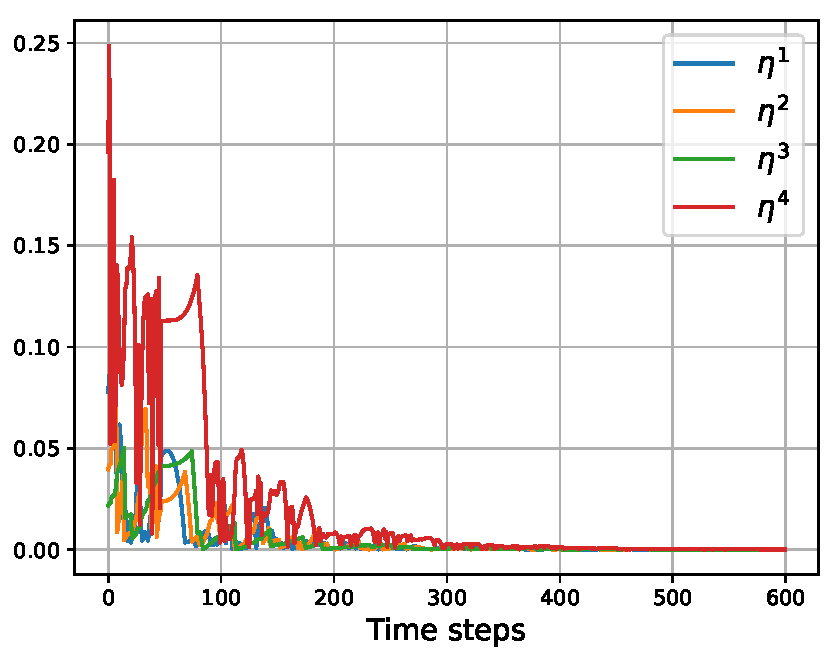
\includegraphics[width=0.45\textwidth]{Figures/eta_plot}
    \caption{First $600$ steps evolution of $\eta^i$ dynamic thresholds}
    \label{fig:eta}
\end{figure}

\begin{figure}[H]
    \centering
    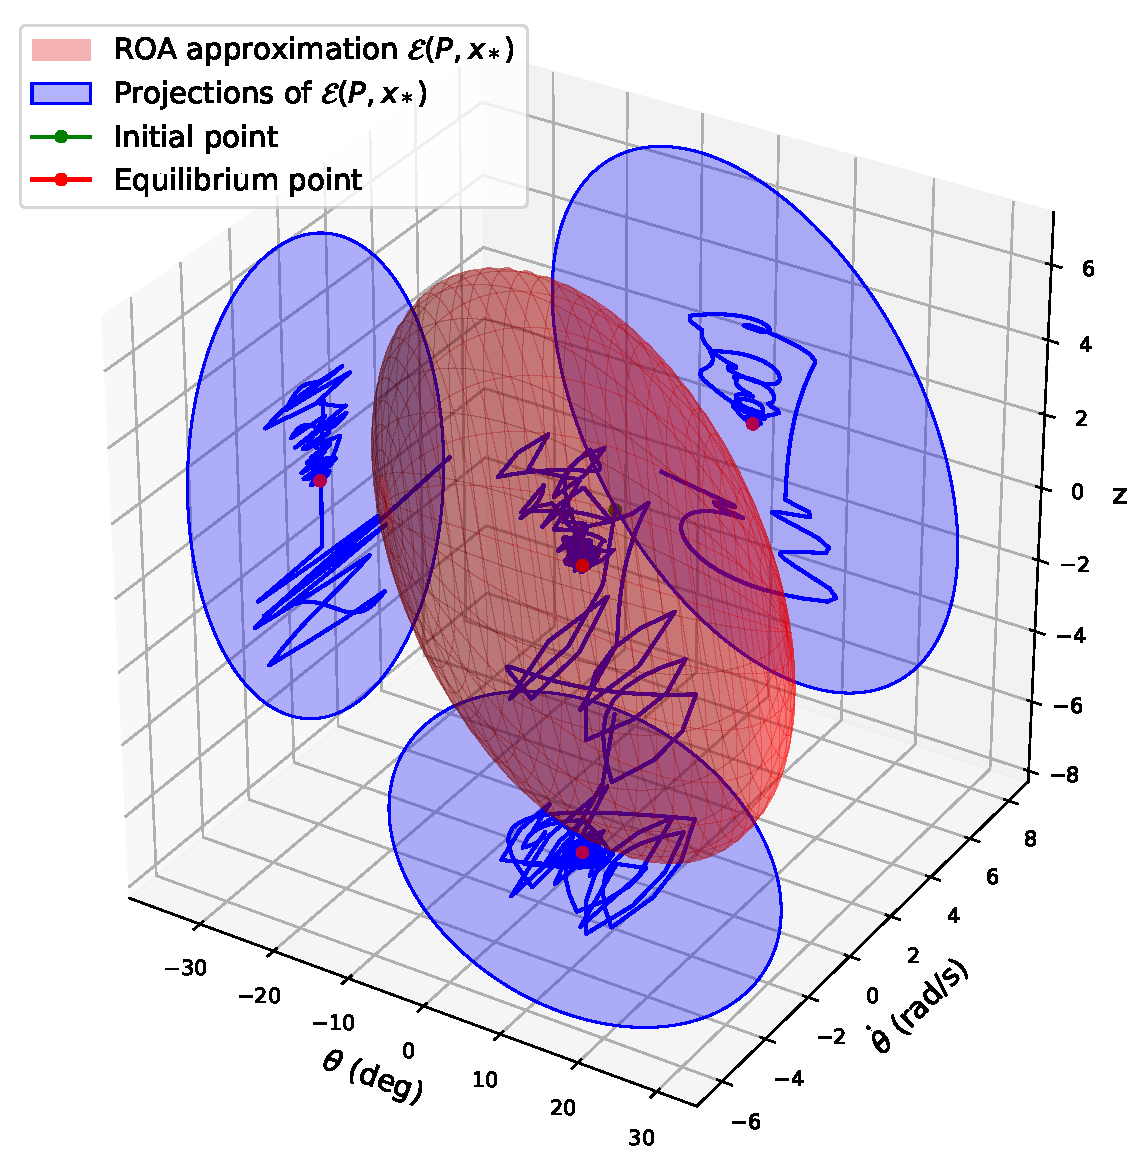
\includegraphics[width=0.45\textwidth]{Figures/ellipsoid_plot}
    \caption{Trajectory of the system within $\cE(P, x_*)$ and with respect to its projections}
    \label{fig:ellipsoid}
\end{figure}


{\color{red} TODO: Chiedi misericordia per l'introduzione}

\section{Conclusions and future works}
In this work, we improved upon the previously published results by addressing a more complex non-linear system controlled by a neural network with more layers, which often leads to a more conservative behavior. Our approach effectively reduced this conservatism, improving the system's performance. Future work will focus on refining Lemma 1 related to Finsler's lemma, specifically to better handle the inclusion where the parameter $\alpha$ appears. Additionally, we plan to explore methods for managing updates close to the equilibrium point, inspired by the concepts introduced in stubborn observer theory.

%\bibliographystyle{plain}
\bibliography{Bibliography/biblio}

\end{document}